\section{Results and Discussion} \label{sec:results}

This section reports validation experiments for debuted genealogical, population size, and positive selection inference techniques.
Results support their efficacy.

\subsection{Genealogical Inference}
\begin{sidewaysfigure}

  \begin{subfigure}{.33\linewidth}
    \centering
    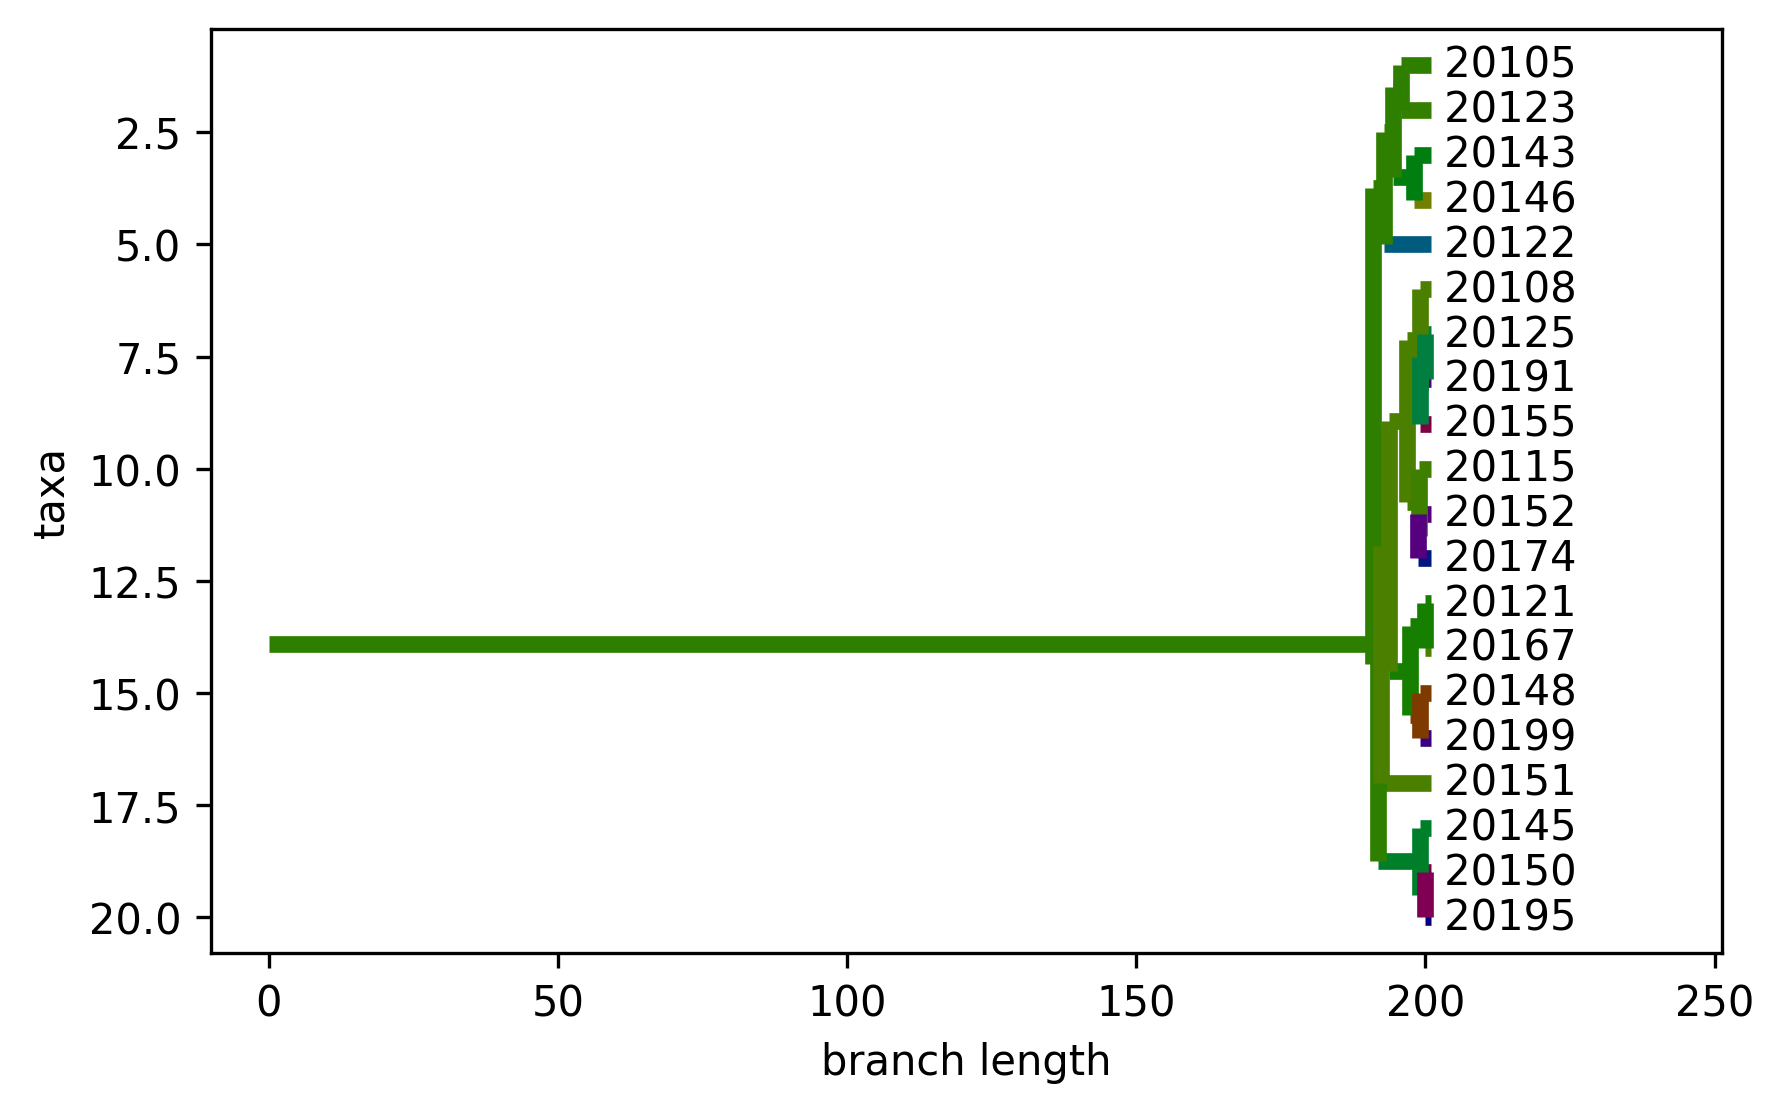
\includegraphics[width=1.05\linewidth]{notebooks/notebooks/teeplots/max_leaves=20+notebook=species-inference+replicate=0+treatment=bag+type=distilled-reference+viz=draw-biopython-tree+ext=}
    \caption{Subcaption 1}
    \label{fig:species-example-replicates:bag-reference}
  \end{subfigure}
  \begin{subfigure}{.33\linewidth}
    \centering
    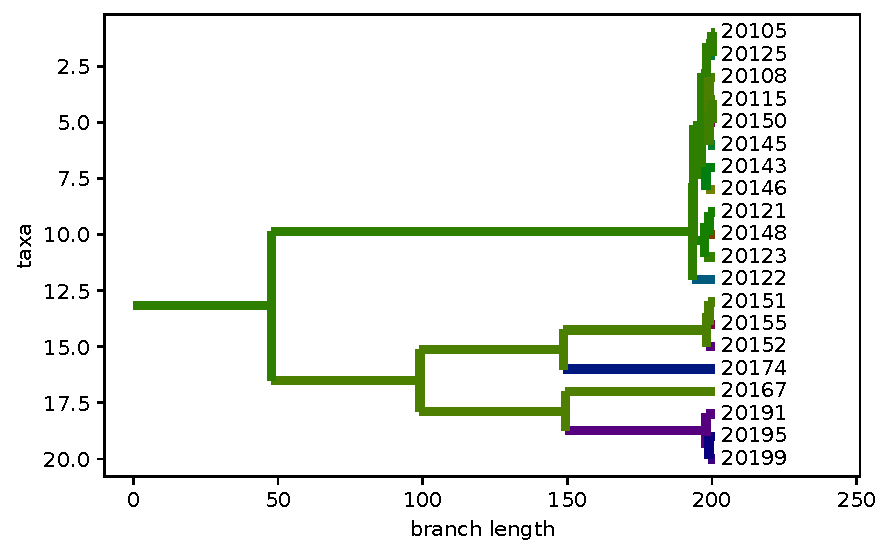
\includegraphics[width=1.05\linewidth]{notebooks/notebooks/teeplots/max_leaves=20+notebook=species-inference+replicate=0+treatment=allopatry+type=distilled-reference+viz=draw-biopython-tree+ext=}
    \caption{Allopatry reference}
    \label{fig:species-example-replicates:allopatry-reference}
  \end{subfigure}
  \begin{subfigure}{.33\linewidth}
    \centering
    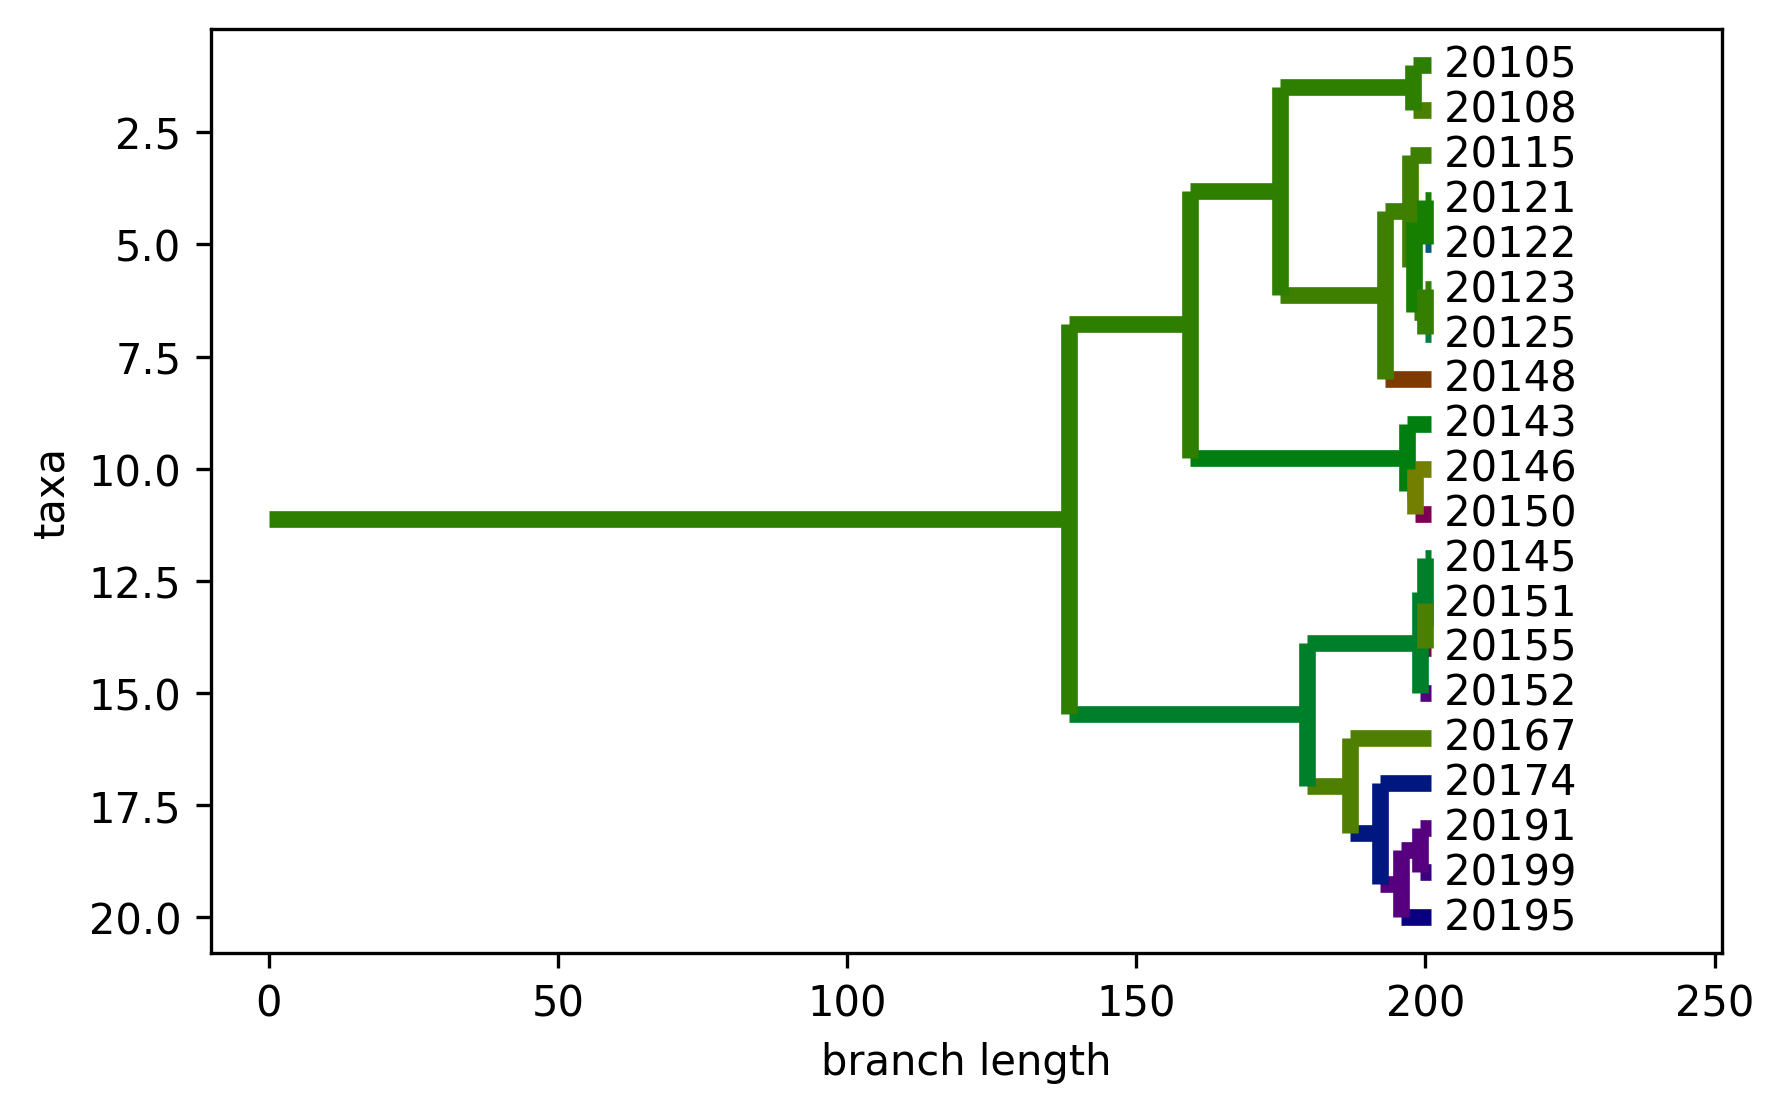
\includegraphics[width=1.05\linewidth]{notebooks/notebooks/teeplots/max_leaves=20+notebook=species-inference+replicate=0+treatment=ring+type=distilled-reference+viz=draw-biopython-tree+ext=}
    \caption{Ring reference}
    \label{fig:species-example-replicates:ring-reference}
  \end{subfigure}

  \begin{subfigure}{.33\linewidth}
    \centering
    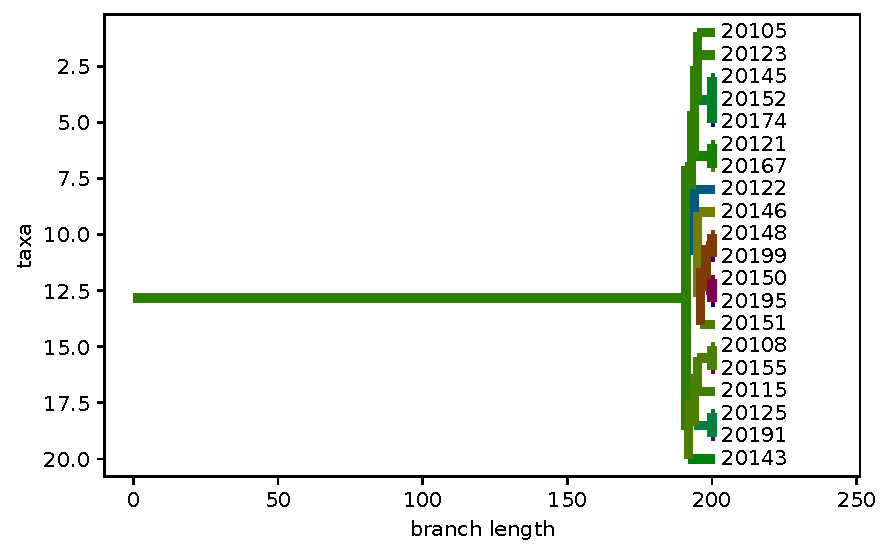
\includegraphics[width=1.05\linewidth]{notebooks/notebooks/teeplots/max_leaves=20+notebook=species-inference+replicate=0+treatment=bag+type=reconstruction+viz=draw-biopython-tree+ext=}
    \caption{Bag reconstruction}
    \label{fig:species-example-replicates:bag-reconstruction}
  \end{subfigure}
  \begin{subfigure}{.33\linewidth}
    \centering
    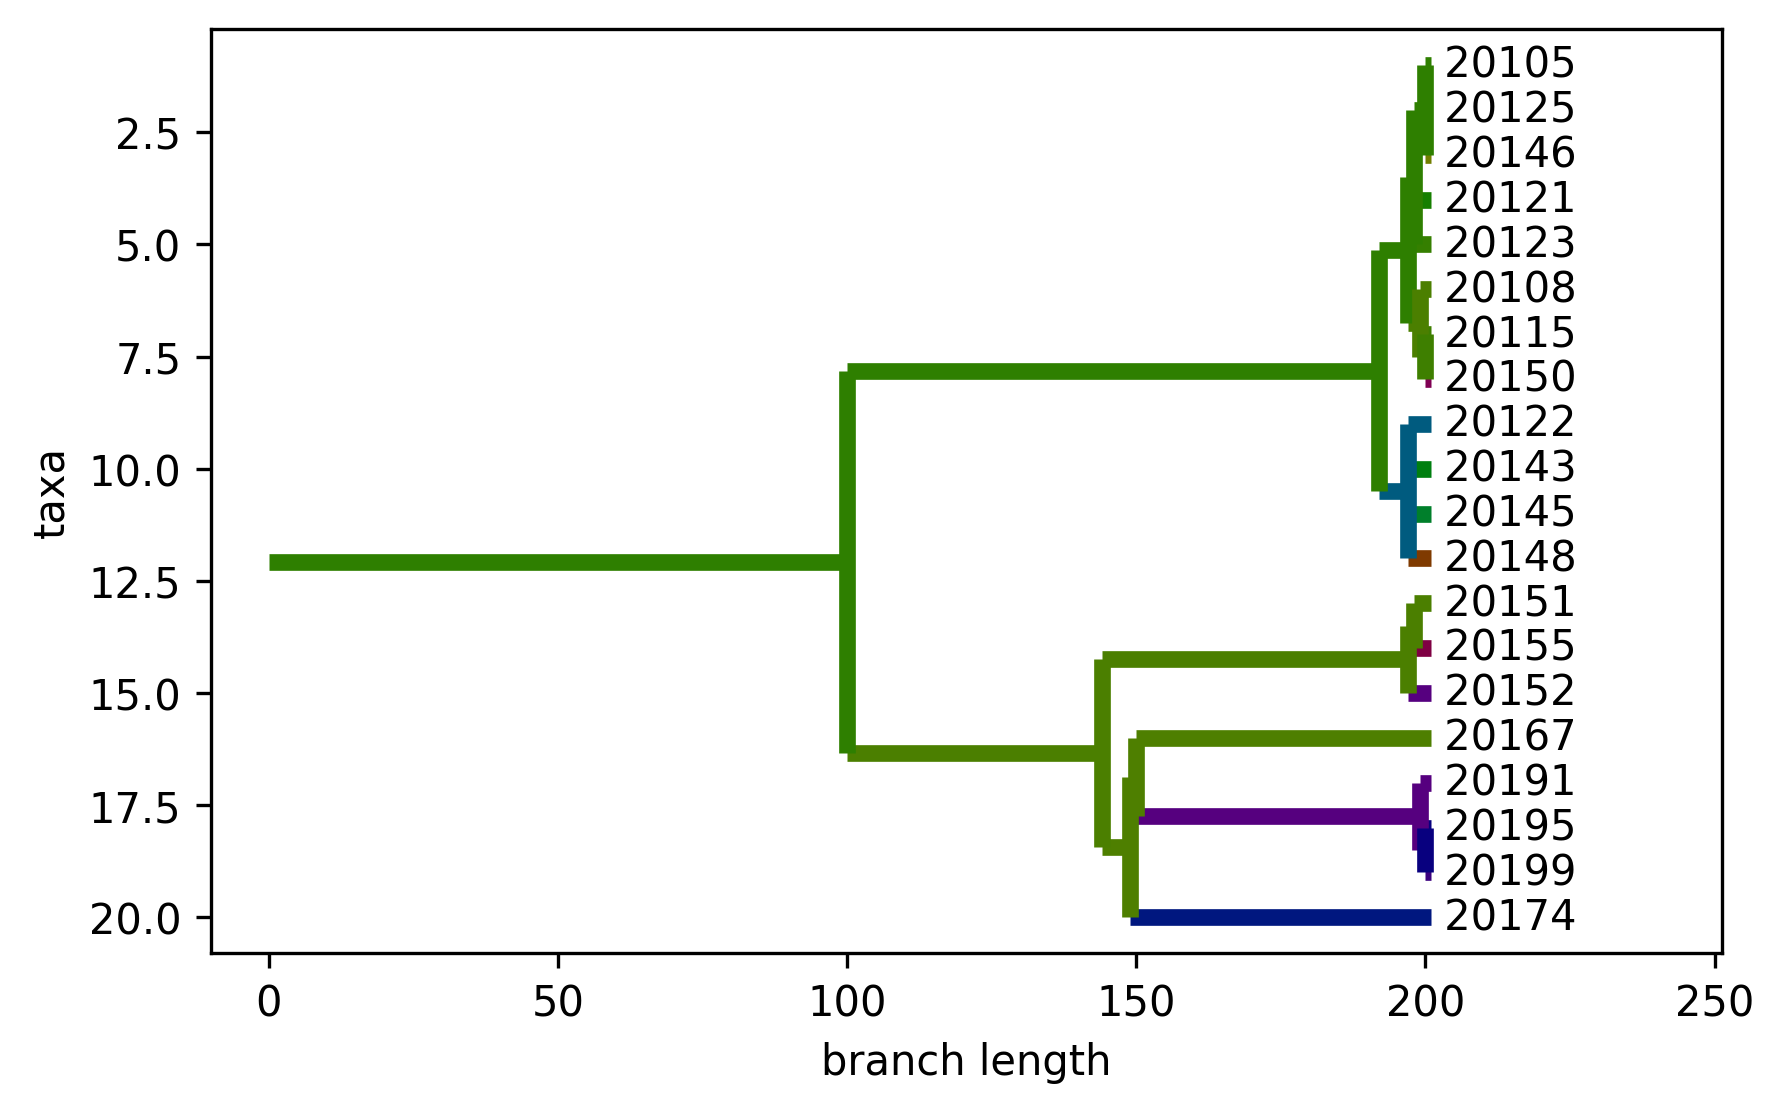
\includegraphics[width=1.05\linewidth]{notebooks/notebooks/teeplots/max_leaves=20+notebook=species-inference+replicate=0+treatment=allopatry+type=reconstruction+viz=draw-biopython-tree+ext=}
    \caption{Allopatry reconstruction}
    \label{fig:species-example-replicates:allopatry-reconstruction}
  \end{subfigure}
  \begin{subfigure}{.33\linewidth}
    \centering
    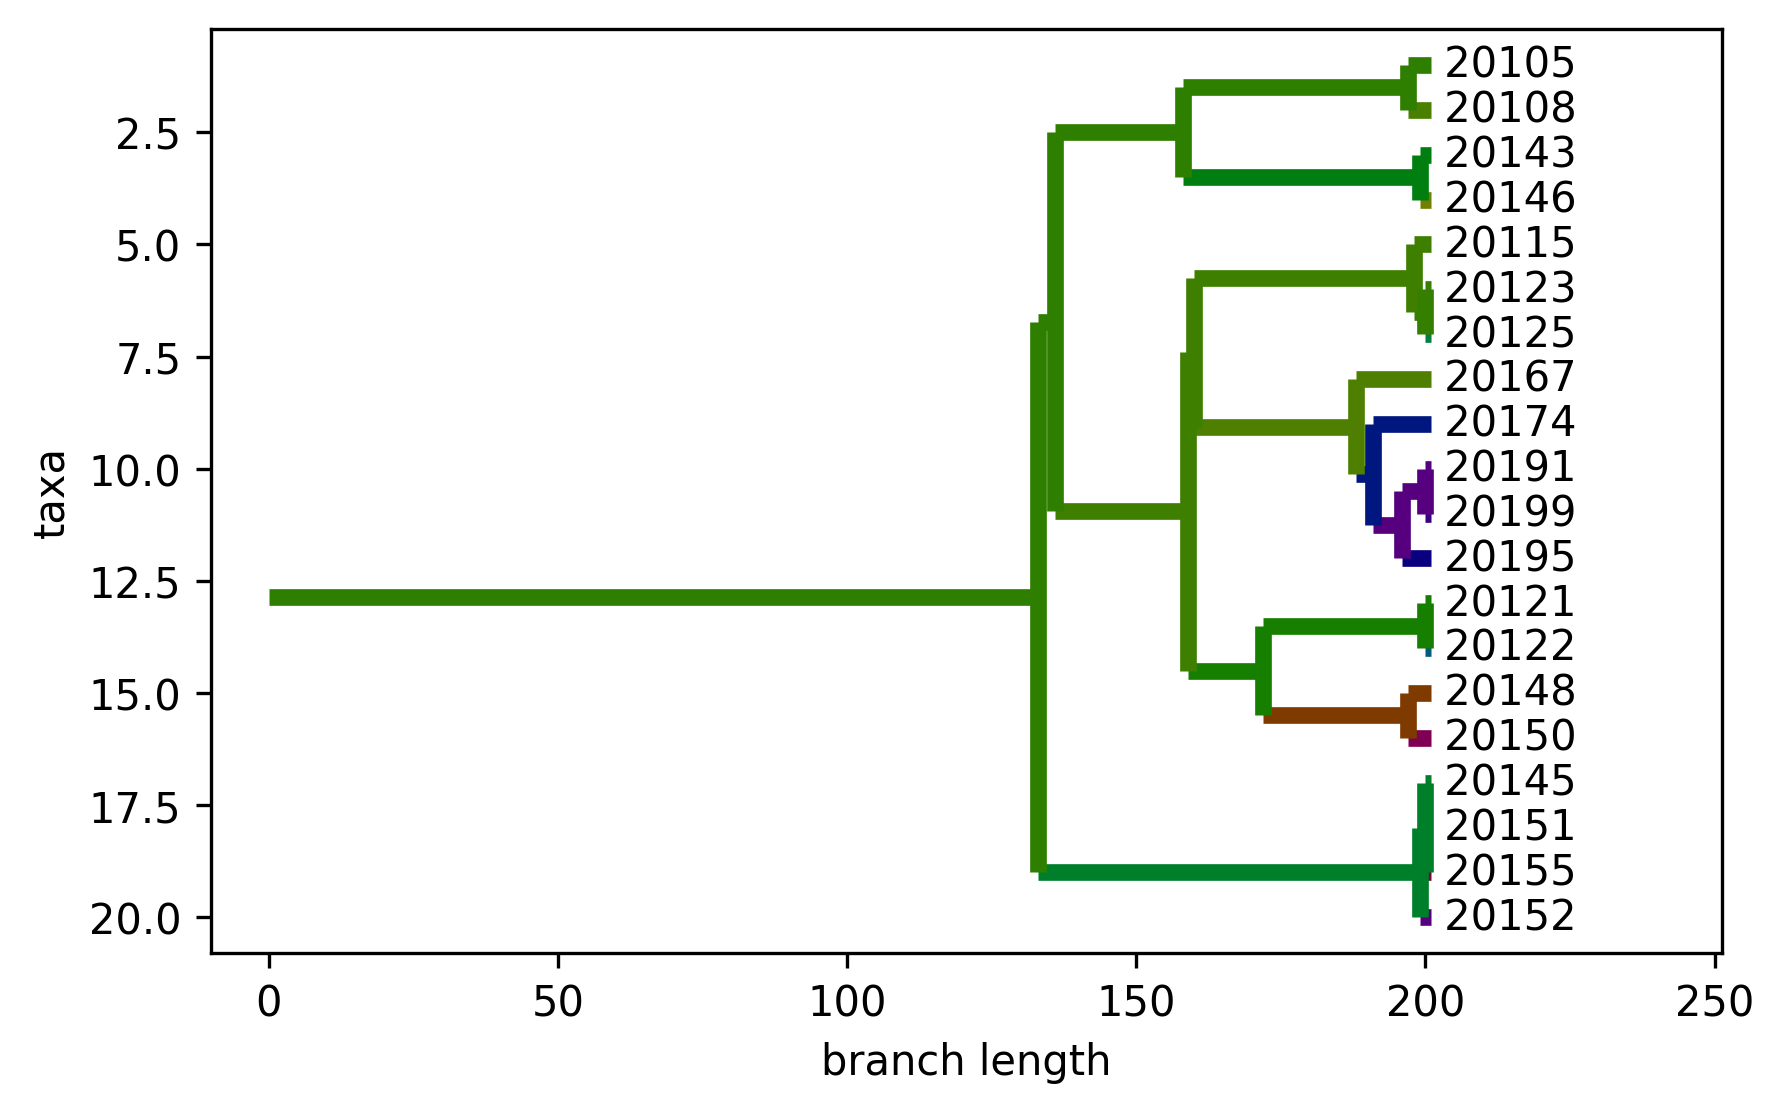
\includegraphics[width=1.05\linewidth]{notebooks/notebooks/teeplots/max_leaves=20+notebook=species-inference+replicate=0+treatment=ring+type=reconstruction+viz=draw-biopython-tree+ext=}
    \caption{Ring reconstruction}
    \label{fig:species-example-replicates:ring-reconstruction}
  \end{subfigure}

  \caption{Caption for the whole figure}
  \label{fig:species-example-replicates}

\end{sidewaysfigure}
%
% notebooks/notebooks/teeplots/max_leaves=20+notebook=species-inference+replicate=0+treatment=allopatry+type=distilled-reference+viz=draw-biopython-tree+ext=.pdf
%
% notebooks/notebooks/teeplots/max_leaves=20+notebook=species-inference+replicate=0+treatment=allopatry+type=reconstruction+viz=draw-biopython-tree+ext=.pdf
%
% notebooks/notebooks/teeplots/max_leaves=20+notebook=species-inference+replicate=0+treatment=bag+type=distilled-reference+viz=draw-biopython-tree+ext=.pdf
%
% notebooks/notebooks/teeplots/max_leaves=20+notebook=species-inference+replicate=0+treatment=bag+type=reconstruction+viz=draw-biopython-tree+ext=.pdf
%
% notebooks/notebooks/teeplots/max_leaves=20+notebook=species-inference+replicate=0+treatment=ring+type=distilled-reference+viz=draw-biopython-tree+ext=.pdf
%
% notebooks/notebooks/teeplots/max_leaves=20+notebook=species-inference+replicate=0+treatment=ring+type=reconstruction+viz=draw-biopython-tree+ext=.pdf

\begin{SCfigure}[3]
  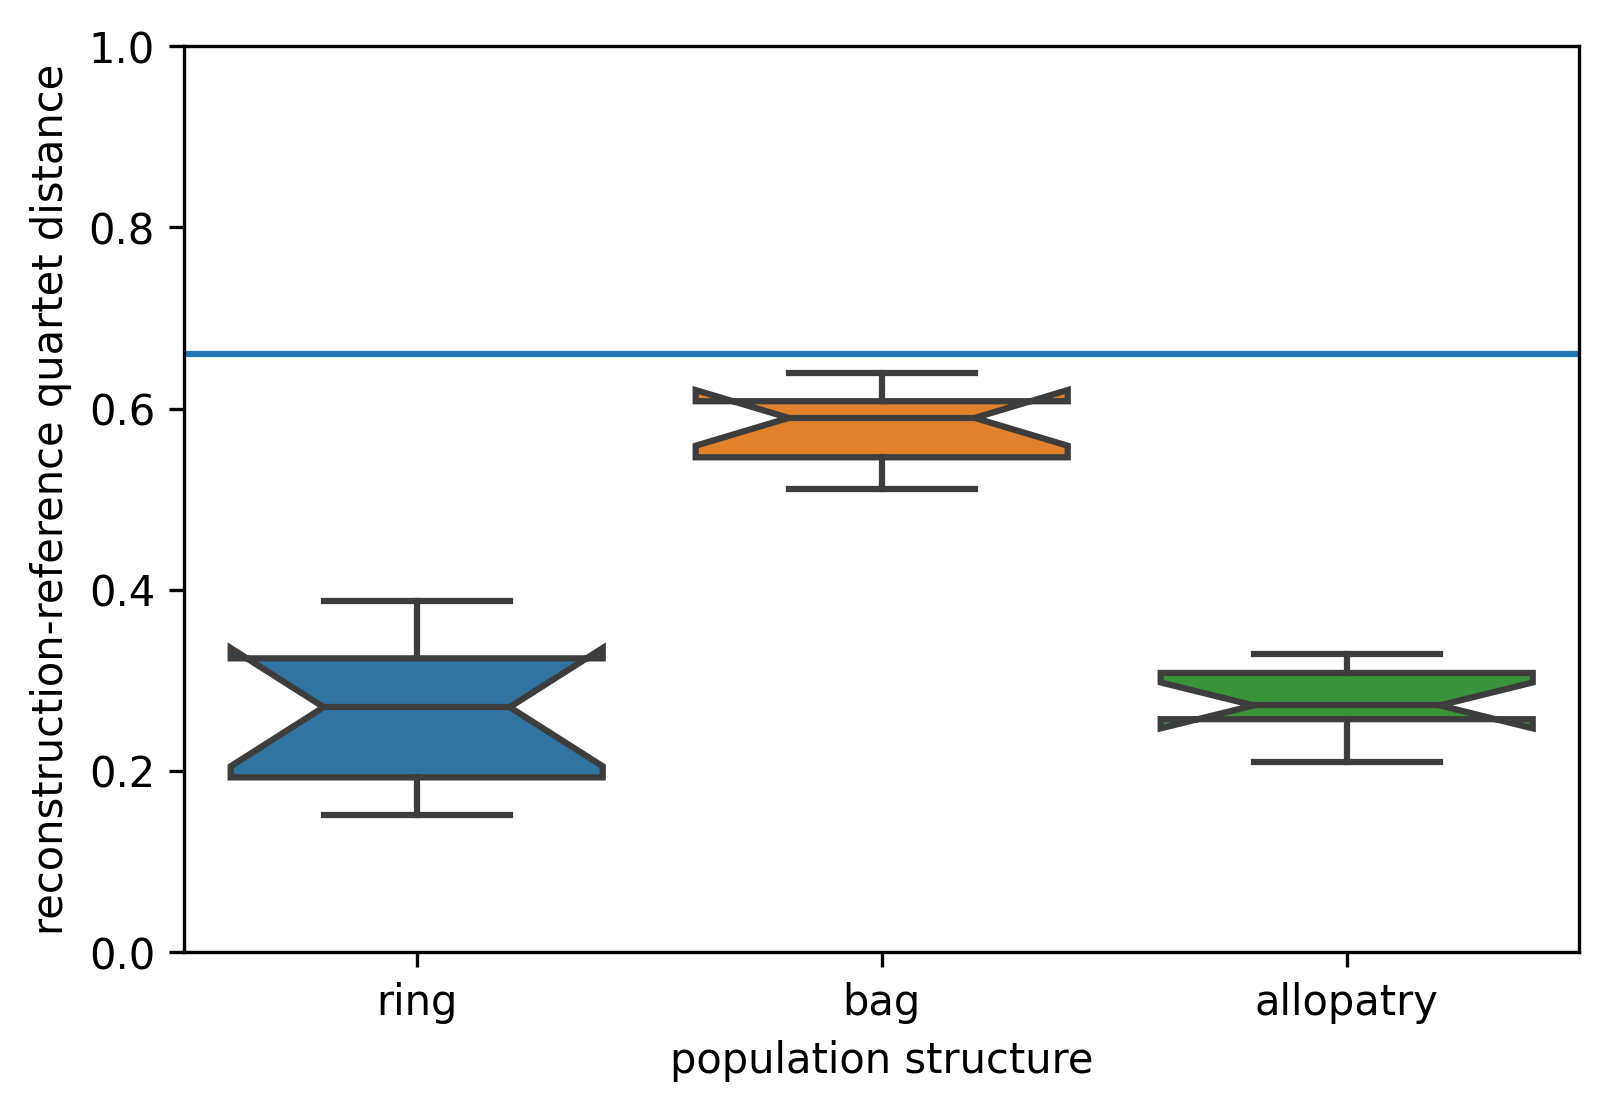
\includegraphics[width=0.5\textwidth]{notebooks/notebooks/teeplots/viz=boxplot-quartet+x=treatment+y=quartet-distance+ext=}
  \caption{
    Normalized quartet distances between reconstructed phylogenies and references distilled from tracked pedigree.
    Lower indicates less reconstruction error.
    Notches give bootstrapped 95\% CI.
    Horizontal blue line indicates expected quartet distance between random trees.
    Some reconstruction error is expected, especially in control treatment, due to resolution of effectively arbitrary phylogenetic structure among well-mixed population components.
  }
  \label{fig:species-reconstruction-error}
\end{SCfigure}


Figure \ref{fig:species-example-replicates} compares phylogenetic trees reconstructed from species-level instrumentation to corresponding references extracted from perfectly-tracked sexual pedigrees.
For treatments with meaningful phylogentic structure --- the ``allopatry'' and ``ring'' treatments --- phylogenetic reconstruction largely succeeded in recovering the historical relationships between subpopulations.
In fact, for the ``allopatry'' treatment, inner node time points appear to more closely track the true generational time frames of speciation events (at generation 100 and 150) than the UPGMA-based pedigree distillation.

Figure \ref{fig:species-reconstruction-error} shows distributions of reconstruction error for each treatment.
Across the three treatments, all ten replicate reconstructions yielded quartet distance from reference below 0.66 (the null expectation for arbitrary trees) \citep{smith2020information}.
This confirms recovery of phylogenetic information in all three cases (exact binomial test, $p < 0.01$).

However, as expected, reconstruction quality on the bag population structure was marginal due to the lack of meaningful phylogenetic information available to reconstruct.
Performance on the ring and allopatry treatments was stronger, achieving quartet distances between reconstruction and reference of around 0.3 in the typical case.
However, junk phylogenetic structure within the reference phylogeny obscures the amount of meaningful reconstruction error.

\subsection{Population Size Inference}
\begin{SCfigure}
  \centering
  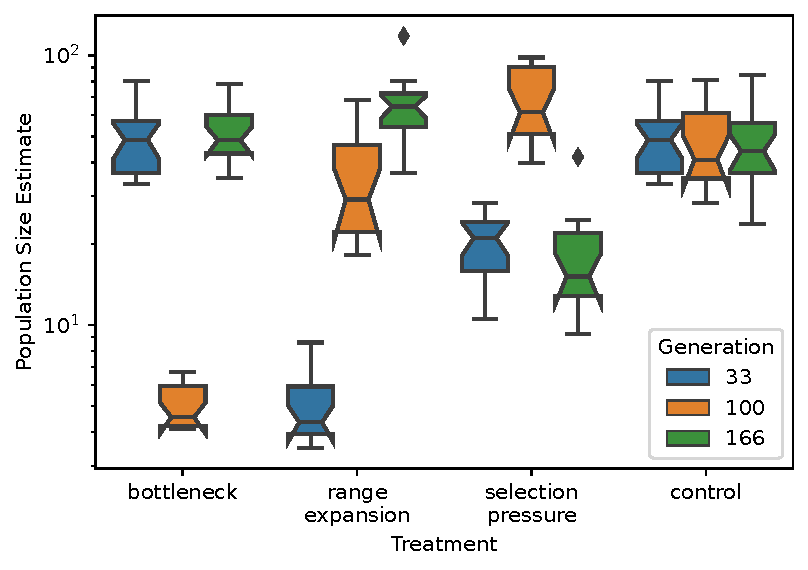
\includegraphics[width=0.6\textwidth]{notebooks/notebooks/teeplots/hue=generation+viz=boxplot-popsize+x=treatment+y=population-size-estimate+ext=}
  \caption{
  Distributions of ten-sample MLE population size estimates by treatment across three time points.
  See Section \ref{sec:population-size-inference} for population size and selection pressure manipulations performed for each treatment.
  Notches indicate bootstrapped 95\% confidence intervals.}
  \label{fig:ne-estimate-distributions}
\end{SCfigure}

% notebooks/notebooks/teeplots/hue=generation+viz=boxplot-popsize+x=treatment+y=population-size-estimate+ext=.pdf


Figure \ref{fig:ne-estimate-distributions} summarizes the distribution of effective population size estimates across replicates at the beginning, middle, and end of evolutionary runs.
Evidencing detection sensitivity, estimates differ across time points within all non-control treatments.
For the bottleneck and selection pressure treatments, which involve reversion to initial conditions, estimate distributions at the first and last time points are comparable, as expected.

Supplemental Figure \ref{fig:ne-example-replicates} shows ten-sample rolling estimates of population size for one replicate from each surveyed treatment.
All population estimates respond to underlying demographic changes, although the response to selection pressure relaxation appears weaker than responses to changes in population size.
Substantial estimate volatility appears across all cases.

Supplemental Figure \ref{fig:ne-detection-matrix} summarizes the detectability of underling effective population size changes.
Detection was performed by evaluating 95\% confidence interval overlap between rolling population size estimates at different time points
No false positives were detected.
Most true changes in effective population size were detected in at least nine out of ten replicates, except for the selection pressure treatment and for the last segment of the range expansion treatment.

\subsection{Positive Selection Inference}
\begin{sidewaysfigure}
  \centering
  \vspace{0.65\textwidth}
  \begin{minipage}{.7\textwidth} % adjust the width as needed

    \begin{minipage}{\textwidth}
      \centering
      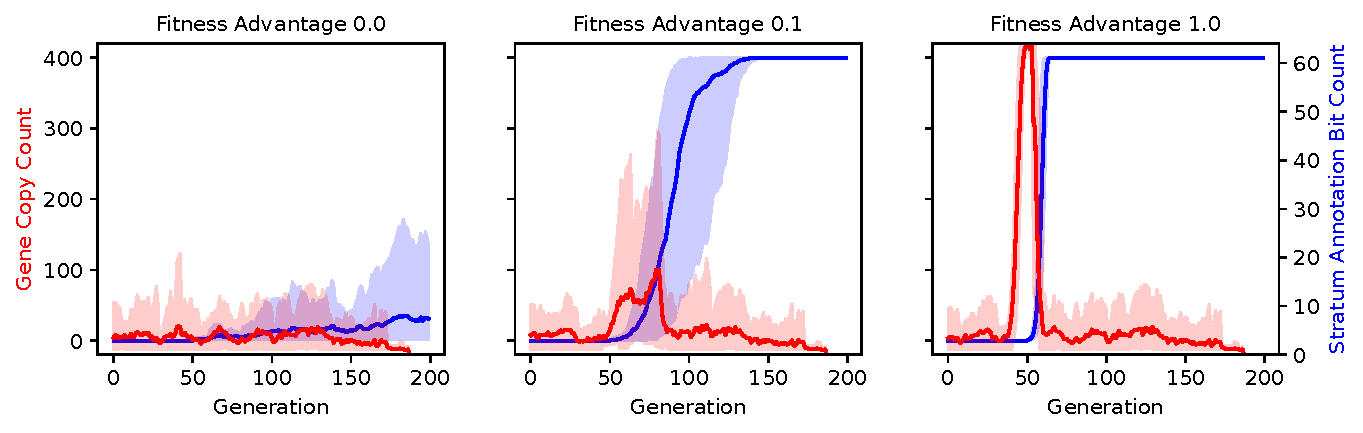
\includegraphics[width=\textwidth]{notebooks/notebooks/teeplots/col=fitness-advantage+viz=facet-lineplot-twiny+x=generation+y1=prevalence+y2=annotation+ext=}
      \subcaption{Cross-replicate aggregate, shaded bands are 95 percentile intervals}
      \label{fig:selection-example-replicates:aggregate}
    \end{minipage}

    \vspace{1cm}

    \centering
    \begin{minipage}{0.32\textwidth}
      \centering
      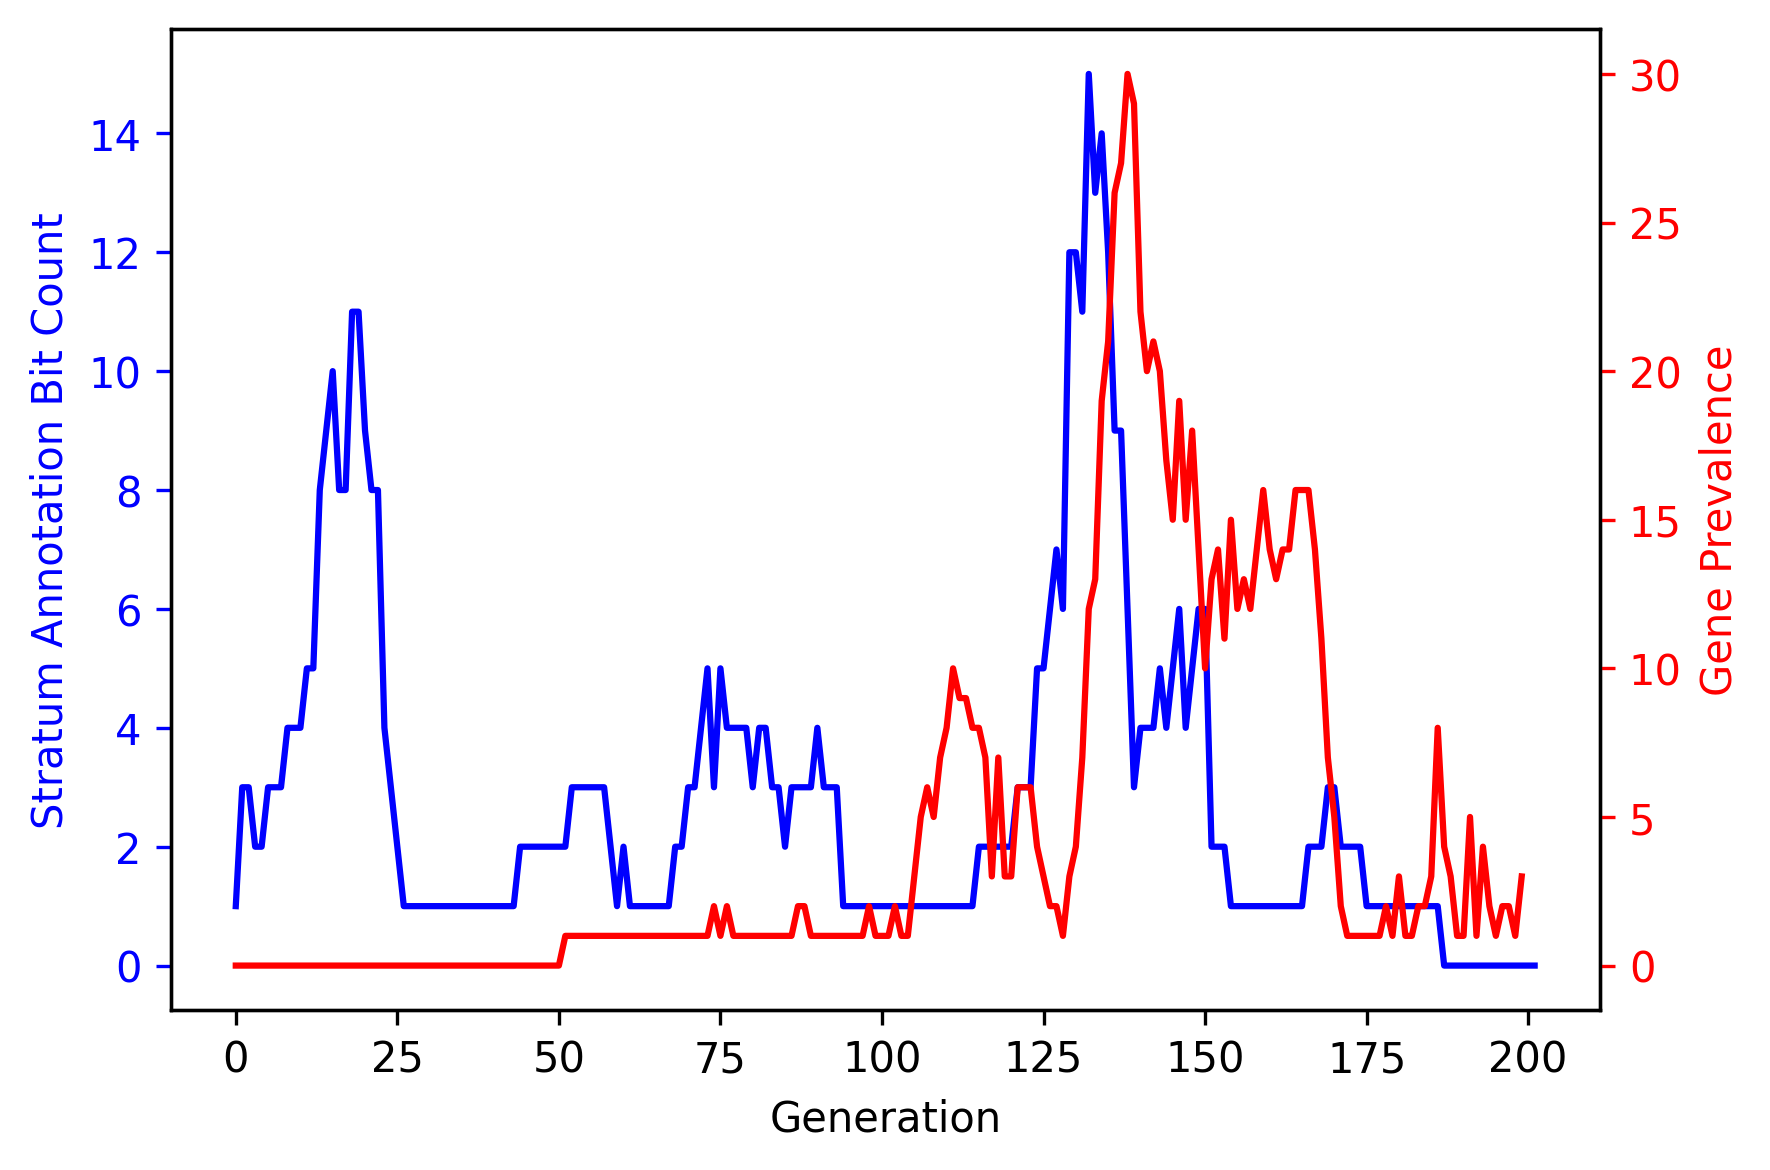
\includegraphics[width=\textwidth]{notebooks/notebooks/teeplots/fitness-advantage=0.0+notebook=gene-selection-inference+replicate=0+viz=plot-sweep-and-annotations+ext=}
      \subcaption{Example replicate with fitness advantage 0.0}
      \label{fig:selection-example-replicates:fit-0-0}
    \end{minipage}
    \begin{minipage}{0.32\textwidth}
      \centering
      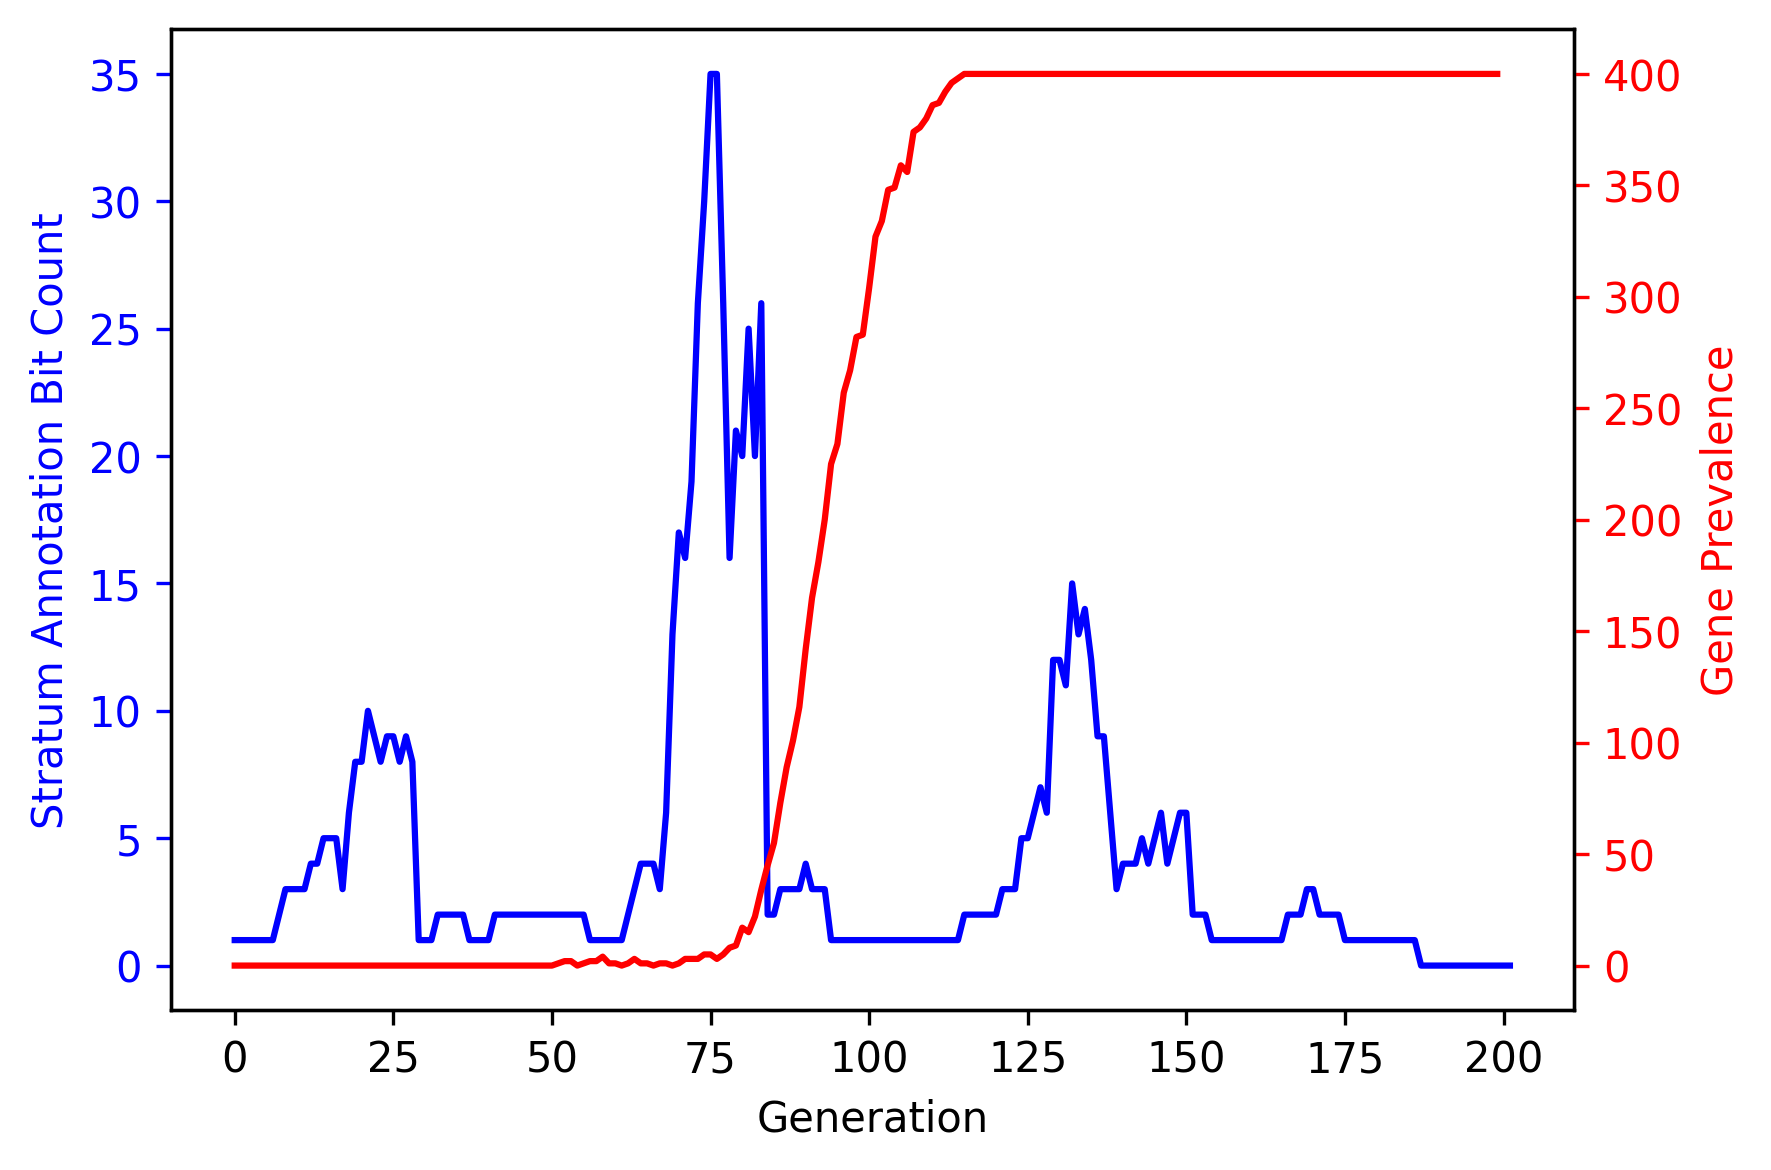
\includegraphics[width=\textwidth]{notebooks/notebooks/teeplots/fitness-advantage=0.1+notebook=gene-selection-inference+replicate=0+viz=plot-sweep-and-annotations+ext=}
      \subcaption{Example replicate with fitness advantage 0.1}
      \label{fig:selection-example-replicates:fit-0-1}
    \end{minipage}
    \begin{minipage}{0.32\textwidth}
      \centering
      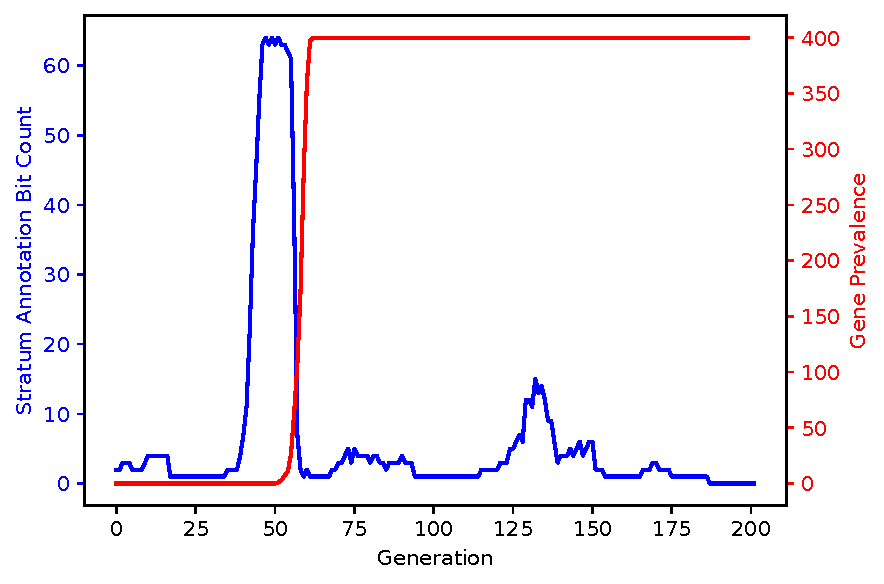
\includegraphics[width=\textwidth]{notebooks/notebooks/teeplots/fitness-advantage=1.0+notebook=gene-selection-inference+replicate=0+viz=plot-sweep-and-annotations+ext=}
      \subcaption{Example replicate with fitness advantage 1.0}
      \label{fig:selection-example-replicates:fit-1-0}
    \end{minipage}%


  \end{minipage}
  \hfill % Creates horizontal space. Can also use \hspace{<len>}
  \begin{minipage}{.25\textwidth} % adjust the width as needed
    \caption{
    Trajectories of true gene prevalence (ired) and instrument set bit counts (blue).
    Top row summarizes distribution across replicates.
    Bottom row shows an example replicate of each treatment.
    Fitness advantage 0.0 conferred no selective benefit.
    Fitness advantage 0.1 corresponded to relatively weak selection and fitness advantage 1.0 corresponded to strong selection.
    Spikes of high gene prevalence annotation bit count (blue) are used to detect underlying selective dynamics (red).
    Note that $y$ axis scaling differs among bottom-row graphs.
    }
    \label{fig:selection-example-replicates}
  \end{minipage}

\end{sidewaysfigure}

Gene selection experiments introduced novel alleles with fitness advantages of 1.0 (strong selection), 0.1 (weaker selection), or 0.0 (no selection --- control).
Figure \ref{fig:selection-example-replicates} plots underlying gene copy count with instrument delay copy count estimates.
These bit counts were extracted from a single randomly-sampled population member.
For the strong selection treatment, allele frequency fixes rapidly and induces a sharp spike in the instrument values.
For the weaker selection treatment, allele frequency grows somewhat less rapidly and is sometimes delayed.
An instrument bit count spike is apparent, but it occurs with a smaller magnitude and more variable timing.

The sensitivity and specificity of positive gene selection detection was evaluated by surveying false-positive (i.e., detection selection on control replicates) and false-negative rates (i.e., non-detection of selection on fitness-advantaged replicates) across a range of detection threshold values.
Supplemental Figure \ref{fig:selection-sensitivity-specificity} plots detection outcomes across a range of detection thresholds.
Strong selection events can be unambiguously distinguished from neutral events, as well as from weaker selection events.
Weaker selection and neutral events were not entirely separable.
The middle-of-the-road detection threshold misidentified one neutral event and one weak positive event --- corresponding to a 10\% false-positive and 10\% false-negative rate.
